\documentclass{article} % For LaTeX2e
\usepackage{nips14submit_e,times}
\usepackage{amsmath}
\usepackage{amsthm}
\usepackage{amssymb}
\usepackage{mathtools}
\usepackage{hyperref}
\usepackage{url}
\usepackage{algorithm}
\usepackage[noend]{algpseudocode}
%\documentstyle[nips14submit_09,times,art10]{article} % For LaTeX 2.09

\usepackage{mathrsfs}
\usepackage{graphicx}
\usepackage{caption}
\usepackage{subcaption}

\def\eQb#1\eQe{\begin{eqnarray*}#1\end{eqnarray*}}
\def\aB#1\aE{\begin{align*}#1\end{align*}}
\def\eQnb#1\eQne{\begin{align}#1\end{align}}
\providecommand{\e}[1]{\ensuremath{\times 10^{#1}}}
\providecommand{\pb}[0]{\pagebreak}

\newcommand{\E}{\mathrm{E}}
\newcommand{\Var}{\mathrm{Var}}
\newcommand{\Cov}{\mathrm{Cov}}

\def\Qb#1\Qe{\begin{question}#1\end{question}}
\def\Sb#1\Se{\begin{solution}#1\end{solution}}

\newenvironment{claim}[1]{\par\noindent\underline{Claim:}\space#1}{}
\newtheoremstyle{quest}{\topsep}{\topsep}{}{}{\bfseries}{}{ }{\thmname{#1}\thmnote{ #3}.}
\theoremstyle{quest}
\newtheorem*{definition}{Definition}
\newtheorem*{theorem}{Theorem}
\newtheorem*{lemma}{Lemma}
\newtheorem*{question}{Question}
\newtheorem*{preposition}{Preposition}
\newtheorem*{exercise}{Exercise}
\newtheorem*{challengeproblem}{Challenge Problem}
\newtheorem*{solution}{Solution}
\newtheorem*{remark}{Remark}
\usepackage{verbatimbox}
\usepackage{listings}
\title{Harmonic Analysis:  \\
Problem Set I}


\author{
Youngduck Choi \\
CIMS \\
New York University\\
\texttt{yc1104@nyu.edu} \\
}


% The \author macro works with any number of authors. There are two commands
% used to separate the names and addresses of multiple authors: \And and \AND.
%
% Using \And between authors leaves it to \LaTeX{} to determine where to break
% the lines. Using \AND forces a linebreak at that point. So, if \LaTeX{}
% puts 3 of 4 authors names on the first line, and the last on the second
% line, try using \AND instead of \And before the third author name.

\newcommand{\fix}{\marginpar{FIX}}
\newcommand{\new}{\marginpar{NEW}}

\nipsfinalcopy % Uncomment for camera-ready version

\begin{document}


\maketitle

\begin{abstract}
This work contains solutions to the problem set I
of Harmonic Analysis 2016 at Courant Institute of Mathematical Sciences.
\end{abstract}

\begin{question}[1]
\hfill
\begin{figure}[h!]
  \centering
    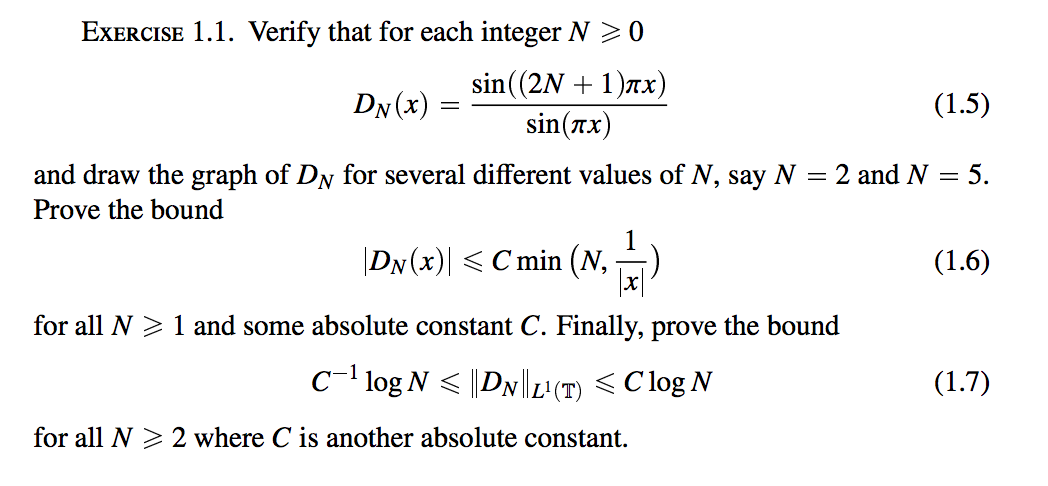
\includegraphics[width=0.8\textwidth]{HA-1-1.png}
\end{figure}
\end{question}

\begin{solution}
We first verify that the given closed form formula for the Dirichlet Kernel $D_n$. Fix 
$x \in \mathbb{T}$ and $N \in \mathbb{N}$. 
From the sum formula for geometric series, and the Euler's identity $
\sin(2\pi nx) = \dfrac{e(-nx) + e(nx)}{2i}$, it follows that 
\eQb
D_{n}(x) &=& \sum_{n=-N}^{N} e(nx) = e(-Nx) \sum_{n=0}^{2N} e(nx) \\
&=& e(-Nx) \dfrac{1 - e((2N+1)x)}{1 - e(x)} = \dfrac{e(-Nx) - e((N+1)x)}{1-e(x)} \\
&=& \dfrac{e(-(N+\frac{1}{2})x - e((N+\frac{1}{2})x)}{e(-\frac{1}{2}x) - e(\frac{1}{2}x)} 
= \dfrac{\sin(2\pi(N+\frac{1}{2})x)}{\sin(2\pi(\frac{1}{2})x)} =
\dfrac{\sin(2(N+1)\pi x)}{\sin(\pi x)},
\eQe
as required.

\pagebreak

 The graphs of $D_2$ and $D_5$ are attached below. The blue graph
corresponds to $D_2$ and the green corresponds to $D_5$.
\begin{figure}[!ht]
  \caption{The graph of $D_n$ for $n=2,5$}
  \centering
    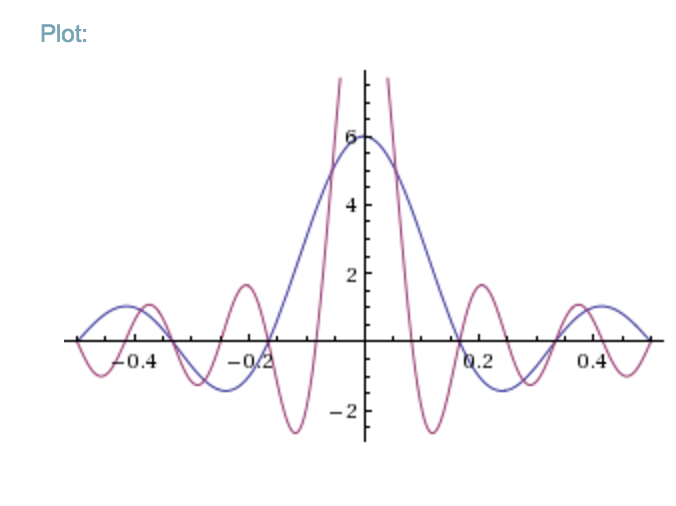
\includegraphics[width=0.5\textwidth]{Dirichlet-plot}
\end{figure}

\smallskip

We proceed to prove the given bound. Fix $x \in \mathbb{T}$ and
$n \in \mathbb{Z}_{+}$. By the triangle inequality, we have
\eQb
\left| D_n(x) \right| &=& \left| \sum_{k=-N}^{N} e(nx) \right| \\ 
&\leq& \sum_{k=-N}^{N} \left| e(nx) \right| = 2N + 1 \leq 3N. \\ 
\eQe

For $ x \in (0,\dfrac{1}{2}]$, we have $2x \leq \sin(\pi x)$. Hence, 
\eQb
\left| D_n(x) \right| 
&=& \left| \dfrac{\sin((2N+1)\pi x}{\sin(\pi x)} \right| = 
 \dfrac{| \sin((2N+1)\pi x| }{ | \sin(\pi x)| } \\
&\leq&  \dfrac{|\sin((2N+1)\pi x)|}{2|x|} \leq \dfrac{1}{2|x|}.
\eQe
Therefore, we obtain that
\eQb
|D_N(x)| &\leq& 3\min(N,\dfrac{1}{|x|}). \\
\eQe

\smallskip

Now, using the monotonicity of Lebesgue integration and additivity over domain gives 
\eQb
||D_N ||_{L^{1}(\mathbb{T})} &=& \int_{\mathbb{T}} |D_n(x)| dx \leq
 \int_{\mathbb{T}} 3\min(N,\dfrac{1}{|x|}) dx \\
&=& 6\int_{0}^{\frac{1}{2}} \min(N,\dfrac{1}{|x|}) dx = 6(\int_{0}^{\frac{1}{N}} N dx
+ \int_{\frac{1}{N}}^{\frac{1}{2}}\dfrac{1}{|x|} dx) \\
&=& 6 + 6(\log(\dfrac{1}{2}) - \log(\dfrac{1}{N}) = 6 + 6\log(\dfrac{1}{2}) + 6\log(N) \leq C_1log(N),
\eQe
where a sufficiently large $C_1$, that satisfies the last inequality when $N = 2$. 
Now, for the lower bound, using the fact that $\sin(\pi x) \leq \pi x$ for $x \in [0,\dfrac{1}{2}]$,
 we have
\eQb
||D_N ||_{L^{1}(\mathbb{T})} &=& \int_{\mathbb{T}} |D_n(x)| dx = 2\int_{0}^{\frac{1}{2}}
|\dfrac{\sin(2N+1)\pi x}{\sin(\pi x)} | dx \\
&\geq& \dfrac{2}{\pi} \int_{0}^{\frac{1}{2}} \dfrac{|\sin(2N+1)\pi x}{x} dx. \\
\eQe
Now, using change of variable with $x = (2N+1)\pi t$, we can continue the computation as follows:
\eQb 
||D_N ||_{L^{1}(\mathbb{T})} 
&\geq& C \int_{0}^{(N+\frac{1}{2})\pi} \dfrac{|\sin(t)|}{t} dt. 
\geq C \int_{0}^{N\pi} \dfrac{|\sin(t)|}{t} dt. \\
&=& C \sum_{i=1}^{N} \int_{(i-1)\pi}^{i\pi} \dfrac{|\sin(t)|}{t} dt. 
\geq C \sum_{i=1}^{N} \dfrac{1}{(i+1)\pi} \int_{(i-1)\pi}^{i\pi} |\sin(t)| dt. \\
&=& C \sum_{i=1}^{N}\dfrac{1}{(i+1)\pi} \cdot \dfrac{\pi}{2}  
\geq C' \sum_{i=1}^{N} \dfrac{1}{i} \geq  C''\log(N),
\eQe
as $\sum_{i=1}^{N} \dfrac{1}{i} \geq c \log(N)$ for some $c$ for $N \geq 2$. Choosing the maximum
$C$ from the upper and the lower bound, we have shown the desired bound on the $L_1$ norm of $D_n$.
\hfill $\qed$
\end{solution}

\bigskip

\begin{question}[2]
\hfill
\begin{figure}[h!]
  \centering
    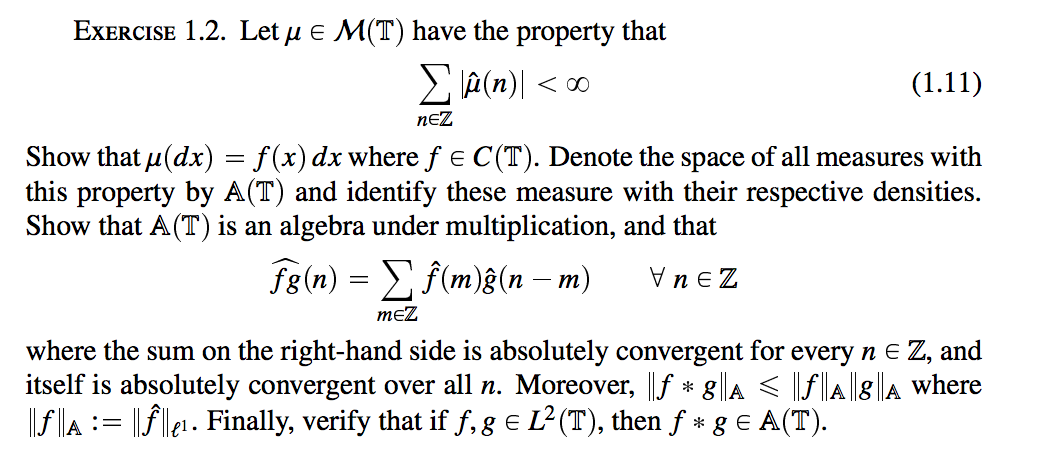
\includegraphics[width=1\textwidth]{HA-1-2.png}
\end{figure}
\end{question}
\begin{solution}

\end{solution}
Let $u \in \mathbb{M}(\mathbb{T})$ 
such that $\sum_{n \in \mathbb{Z}} |\hat{u}(n)| < \infty$. By the Lebesgue-Radon-Nikodym
theorem (Rudin pg.121), there exists $f \in L_1(\mathbb{T})$ such that $u(dx) = f(x)dx$,
where $dx$ is the Lebesgue measure, restricted to Borel sets of $\mathbb{T}$. Let $f$ be
such function in $L_1(\mathbb{T})$. As 
$u(dx) = f(x)dx$, it follows that $\hat{u}(n) = \hat{f}(n)$, thus $\sum_{n \mathbb{Z}} 
|\hat{f}(n)| < \infty$. We claim that $f$ is continuous. Fix $\epsilon > 0$. Hence,
this show that $f \in \mathbb{C}(\mathbb{T})$ as desired. This shows that
$\mathbb{A}(\mathbb{T})$ is an algebra under multiplication. 
\eQb
fg &\sim& \sum_{n = -\infty}^{\infty} \sum_{m \in \mathbb{Z}} \hat{f}(m) \hat{g}(n-m) e(nx)   
\eQe

Let $f,g \in L^{2}(\mathbb{T})$. 
\newpage

\begin{question}[3]
\hfill
\begin{figure}[h!]
  \centering
    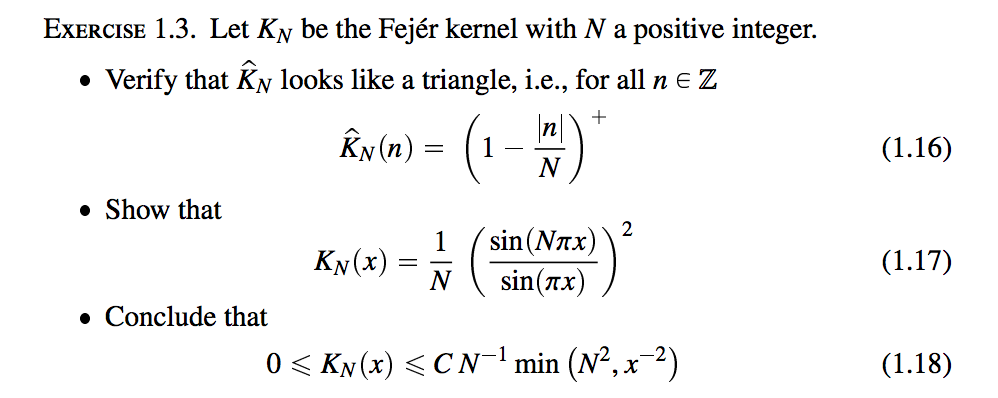
\includegraphics[width=1\textwidth]{HA-1-3.png}
\end{figure}
\end{question}
\begin{solution} Let $K_N$ be the Fejer kernel with the positive integer $n$. \\

\smallskip

\textbf{(1.16)} 
From definition of $n$th Fourier coefficient, we obtain
\eQb
\hat{K}_{N}(n) &=& \int_{\mathbb{T}} K_n(x)e(-nx) dx 
= \int_{\mathbb{T}} (\dfrac{1}{N} \sum_{k=0}^{N-1} D_k(x)) e(-nx) dx \\
&=& \int_{\mathbb{T}} \dfrac{1}{N} \sum_{k=0}^{N-1} \sum_{|m| \leq k} e(mx) e(-nx) dx 
= \dfrac{1}{N} \sum_{k=0}^{N-1} \sum_{|m| \leq k} 
\int_{\mathbb{T}} e((m-n)x) dx. \\
\eQe
Observe that the integral in the summation is $1$ if $m = n$ and $0$ otherwise. For $n \leq N$,
we have $(N - |n|)$ terms in the sum where $m = n$ happens, for $n > N$, we have no such term, where 
the equality holds. Therefore, it follows that
\eQb
\hat{K}_{N}(n) &=& \dfrac{1}{N}(N - |n|)^{+} = (1 - \dfrac{|n|}{N})^{+},
\eQe
which is precisely the given closed form formula for the kernel. \hfill $\qed$

\bigskip

\textbf{(1.17)}
Fix $x \in \mathbb{T}$, and $N \in \mathbb{N}$.
Now, by definition of Fejer Kernel, we have
\eQb
K_N(x) &=& \dfrac{1}{N} \sum_{n=0}^{N-1} D_n(x) 
= \dfrac{1}{N} \sum_{n=0}^{N-1} \dfrac{\sin((2n+1)\pi x)}{\sin(\pi x)} \\
&=& \dfrac{1}{N\sin(\pi x)^2}\sum_{n=0}^{N-1} \sin((2n+1)\pi x)\sin(\pi x). \\
\eQe
By the use of the trig identity, $\sin(a)\sin(b) = \dfrac{1}{2}\cos(a-b) - \cos(a+b)$, and
cancellation from a telescoping sum, it follows that
\eQb
K_N(x) &=& \dfrac{1}{2N\sin(\pi x)^2}\sum_{n=0}^{N-1}
(\cos(2n \pi x) - \cos((2n + 2)\pi x)) \\
&=& \dfrac{1}{2N\sin(\pi x)^2}(1 - \cos(2N\pi x)) \\
\eQe
Lastly, from the trig identity, $2\sin(a)^2 = 1 - \cos(2a)$, we finally obtain that
\eQb
K_N(x) &=& \dfrac{1}{2N\sin(\pi x)^2}(2\sin(N\pi x)^2)
= \dfrac{1}{N}(\dfrac{\sin(N\pi x)}{\sin(\pi x)})^2,
\eQe
as required. 

\bigskip

\textbf{(1.18)} Fix $x \in \mathbb{T}$, and $N \in \mathbb{N}$. From $(1.17)$, it is
clear that $0 \leq K_n(x)$. By the triangle inequality, and the result from the excercise $1.1$,
it follows that
\aB 
K_N(x) &\leq \dfrac{1}{N} \sum_{n=0}^{N-1}| D_n(x) | 
\leq \dfrac{1}{N} \sum_{n=0}^{N-1} 2n + 1 = \dfrac{1}{N} (2\dfrac{N(N-1)}{2} + N) = N \notag  
\aE
Now, by the $(1.17)$ result, and the fact that $|\sin(x)| \leq 2|x|$ for $x \in [0,\dfrac{1}{2}]$,
 we obtain
\eQb
K_N(x) &=& \dfrac{1}{N}(\dfrac{\sin(N \pi x)}{\sin(\pi x)})^2 
\leq \dfrac{1}{N}(\dfrac{\sin(N \pi x)}{2x})^2  
\leq \dfrac{1}{N} \cdot \dfrac{1}{4x^2} \leq \dfrac{1}{Nx^2}.
\eQe
Hence, we have shown that 
\eQb
0 &\leq& K_n(x) \leq N^{-1} \min(N^2,\dfrac{1}{x^2}),
\eQe
as required.

\hfill $\qed$

\end{solution}

\bigskip

\begin{question}[4]
\hfill
\begin{figure}[h!]
  \centering
    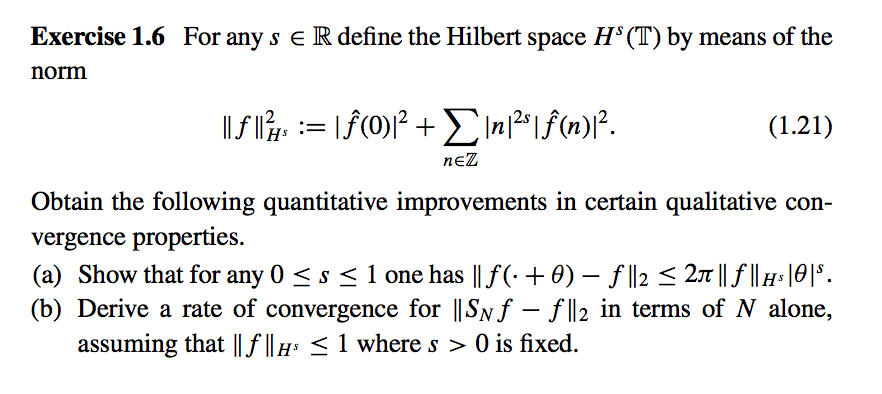
\includegraphics[width=1\textwidth]{HA-1-4.png}
\end{figure}
\end{question}
\begin{solution} \hfill \\
\textbf{(a)} Let $0 \leq s \leq 1$, and $h = \tau_{-\theta}f$, where $\tau_{\theta}f(x)
= f(x-\theta) $
is the translation operator, parametrized by $\theta$. 
By the Corollary $1.6$,
and the linearity of integration, it follows that
\eQb
||h - f||_2^2 &=& \sum_{-\infty}^{\infty} |\widehat{(h-f)}(n)|^2  \\
&=& \sum_{-\infty}^{\infty} |\hat{h}(n) - \hat{f}(n)|^2. 
\eQe 
Now, we have a particular relation between the Fourier transform 
and translation as follows (pg. 4 in Schleg): 
\eQb
\widehat{{\tau}_{-\theta}f}(n) = e(n \theta)\hat{f}(n).
\eQe
Hence, it follows that
\eQb
|| h - f||_{2}^2 &=&  \sum_{-\infty}^{\infty} |e(n \theta) \hat{f}(n) - \hat{f}(n)|^2 \\
&=& \sum_{-\infty}^{\infty} |e(n \theta) - 1|^2 |\hat{f}(n)|^2 \\
\eQe
Recall that $\theta \in [0,1)$ and $0 \leq s \leq 1$. For $|n \theta| \geq 1$, we have
\eQb
|e(n \theta ) - 1|^2 &\leq& 4 \leq  4\pi^2 |n|^{2s} |\theta|^{2s}. \\ 
\eQe
Now, when $|n \theta | <1$, by rudimentary trig identities, we obtain 
\eQb
|e(n \theta ) - 1|^2 &\leq& (\cos(2\pi n \theta)^2 -1)^2 + \sin(2\pi n \theta)^2 \\
&=& 2 - 2\cos(2\pi n \theta) =  4\sin^2(\pi n \theta) \\ 
&\leq& 4\pi^2 n^{2} |\theta|^2 \leq  4\pi^2 |n|^{2s} |\theta|^{2s}. 
\eQe

\bigskip

Hence, we have shown
$|e(n \theta ) - 1|^2 \leq  4\pi^2 |n|^{2s} |\theta|^{2s}$.  
Plugging the above inequality into the two norm inequality above gives
\eQb
|| h - f||_{2}^2 &\leq&  
4\pi^2 \big( \sum_{-\infty}^{\infty} n^2 \hat{f}(n)|^2 \big) |\theta|^{2s}\\
&\leq& 4\pi^2 ||f||_{H^s(\mathbb{T})}^2 |\theta|^{2s},
\eQe
and consequently,
\eQb 
||h - f||_2 &\leq& 2\pi ||f||_{H^s(\mathbb{T})}|\theta|^{s},
\eQe
as required.

\bigskip

\textbf{(b)} Fix $s > 0$. By definition of $S_N f$, and the given, we have
\eQb
||S_N f - f||_{2}^{2} = \sum_{|n| > N} |\hat{f}(n)|^2
 &\text{and }& \> ||f||_{L^2} \leq ||f||_{H^s} \leq 1
\eQe
With the given norm, it follows that
\eQb
1 &\geq& ||f||_{H^s} \\
&\geq& \sum_{|n| > N} (N+1)^{2s}|\hat{f}(n)|^2 = (N+1)^{2s} ||S_N f - f||_{2}^{2},\\
\eQe
which can be simplified to  
\eQb
||S_N f - f||_{2} &\leq& \dfrac{1}{(N+1)^{2s}}, 
\eQe
which reveals the rate of convergence as required.
\hfill $\qed$
\end{solution}

\bigskip

\begin{question}[5]
\hfill
\begin{figure}[h!]
  \centering
    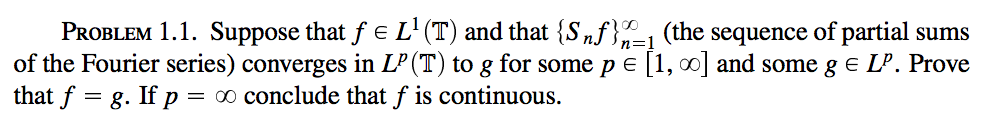
\includegraphics[width=1\textwidth]{HA-1-5.png}
\end{figure}
\end{question}
\begin{solution}
Let $p \geq 1$. Observe that for $x \in [0,1)$, we have $|x| \leq |x|^p$. Hence, it follows that
\eQb
0 \leq \int_{\mathbb{T}} |S_nf - g| \leq \int_{\mathbb{T}} |S_n f - g|^p. 
\eQe
As we are given that $\int_{\mathbb{T}} |S_n f - g|^p \to 0$ as $n \to \infty$
it follows that $\int_{\mathbb{T}} |S_n f - g| \to 0$ in $L^1(\mathbb{T})$.  
\end{solution}

\bigskip

\begin{question}[6]
\hfill
\begin{figure}[h!]
  \centering
    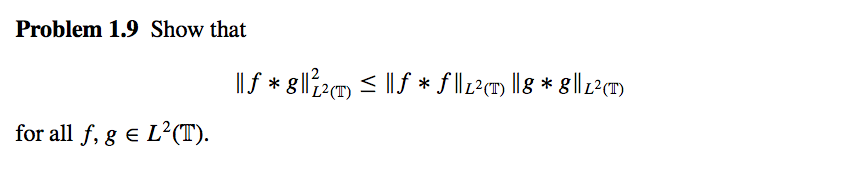
\includegraphics[width=1\textwidth]{HA-1-6.png}
\end{figure}
\end{question}
\begin{solution}
As we have $f,g \in L^2(\mathbb{T})$, by Corollary $1.6$, the given inequality is equivalent to
\eQb
\sum_{n \in \mathbb{Z}} |\widehat{f * g}(n)|^2 &\leq&
\sqrt{\sum_{n \in \mathbb{Z}} |\widehat{f * f}(n)|^2}  
\sqrt{\sum_{n \in \mathbb{Z}} |\widehat{g * g}(n)|^2}. \\
\eQe
Since $\widehat{f*g}(n) = \hat{f}(n)\hat{g}(n)$, the above inequality is again equivalent to
\eQb
\big( \sum_{n \in \mathbb{Z}} |\hat{f}(n)\hat{g}(n)|^2 \big)^2 &\leq&
\sum_{n \in \mathbb{Z}} |\hat{f}(n)|^4 
\sum_{n \in \mathbb{Z}} |\hat{g}(n)|^4. \\
\eQe
Expanding the LHS of the desired inequality yields
\eQb
\big( \sum_{n \in \mathbb{Z}} |\hat{f}(n)\hat{g}(n)|^2 \big)^2 &=&
\sum_{n \in \mathbb{Z}} |\hat{f}(n)\hat{g}(n)|^4 + 
\sum_{n > m} 2|\hat{f}(n)\hat{f}(m)\hat{g}(n)\hat{g}(n)|^2 \\
&\leq&
\sum_{n \in \mathbb{Z}} |\hat{f}(n)\hat{g}(n)|^4 + 
\sum_{n > m} |\hat{f}(n)\hat{g}(n)|^4 + |\hat{f}(m)\hat{g}(m)|^4 \\
&=& \sum_{n \in \mathbb{Z}} |\hat{f}(n)|^4 
\sum_{n \in \mathbb{Z}} |\hat{g}(n)|^4, \\
\eQe
where the last inequality
holds by the Cauchy-Schwarz inequality on the inner product space of $l^2(\mathbb{T})$.

\hfill $\qed$ 
\end{solution}

\bigskip

\begin{question}[Extra]
\hfill
\begin{figure}[h!]
  \centering
    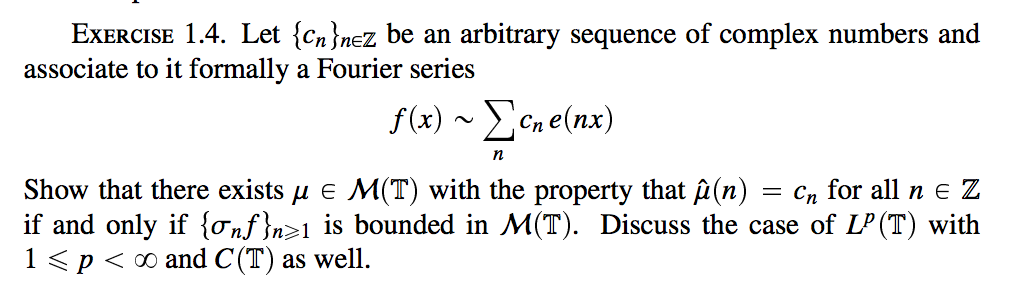
\includegraphics[width=1\textwidth]{HA-1-Extra.png}
\end{figure}
\end{question}
\begin{solution}
\end{solution}
\end{document}
